\documentclass[dvipdfmx]{jarticle}
\pagestyle{empty}
\include{cmacros}
\begin{document}
\begin{tikzpicture}
 \cstat{a$_1$=1;}
 \cstat{b$_1$=2;}
 \cstat{x$_1$=3;}
 \cstat{y$_1$=a$_1$+b$_1$;}
 \cstat{c$_1$=x$_1$+y$_1$;}
 \cstat{if(a$_1$<10)}
 \cstatl{z$_1$=a$_1$+b$_1$;}
 \cstat{else}
 \cstatl{z$_2$=a$_1$+b$_1$;}
 \cstat{z$_3$=$\phi$(z$_1$,z$_2$);}
 \cstat{d$_1$=x$_1$+z$_3$;}
 \cstat{println(d$_1$);}
\end{tikzpicture}
\end{document}
